\section{}
Using Castigliano's theorem, find the slope of the deflection curve at midlength C of a beam due to 
applied couple moment $M_0$ Fig. \ref{fig:Q4ProblemDiagram}.

\begin{figure}[h]
    \centering
    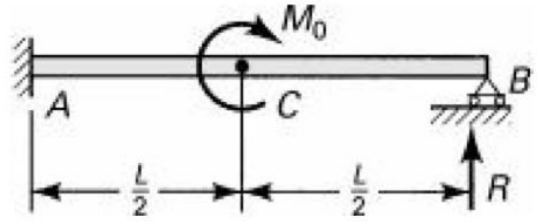
\includegraphics[width=0.5\linewidth]{Questions/Figures/Q4ProblemDiagram.png}
    \caption{Propped cantilever beam AB}
    \label{fig:Q4ProblemDiagram}
\end{figure}

First, the reaction force R needs to be determined. The moment equation from B to A is:
\begin{align*}
    M &= Rx - M_0 \langle x-  \frac{L}{2} \rangle^0, \quad \langle x-  \frac{L}{2} \rangle^0 = H\left(x - \frac{L}{2}\right) \\
    \implies \frac{\partial M}{\partial R} &= x \\
    \implies \frac{\partial M}{\partial M_0} &= -\langle x-  \frac{L}{2} \rangle^0 
\end{align*}

By Castigliano's theorem, the deflection at B is:
\begin{align*}
    \delta_B &= \frac{1}{EI} \left[\int_{0}^{L/2} Rx^2 dx - \int_{L/2}^{L} Rx^2 - M_0x dx \right] \\
    &= \frac{1}{EI} \left[\frac{RL^3}{24} - \frac{L^2(9M_0 - 7LR)}{24} \right] 
\end{align*}

Since the pin at B cannot carry deflection, $\delta_B = 0$. Therefore,
\begin{align*}
    \delta_B \overset{\text{set}}{=} 0 &= \frac{1}{EI} \left[\frac{RL^3}{24} - \frac{L^2(9M_0 - 7LR)}{24} \right] \\
    \implies R &= \boxed{\frac{9M_0L}{8 L}}
\end{align*}    

To find the slope at C, apply Castigliano's theorem again:
\begin{align*}
    \theta_C &= \frac{1}{EI} \left[\cancel{\int_{0}^{L/2} M \left(\frac{\partial M}{\partial M_0}\right) dx}
     + \int_{L/2}^{L} M \left(\frac{\partial M}{\partial M_0}\right) dx \right] \\
    &= \frac{1}{EI} \int_{L/2}^{L}  M_0 - Rx dx \\
    &= \frac{4 M_0L - 3RL^2}{8EI} \\
    &= \boxed{\frac{5LM_0}{64EI}}
\end{align*}